Here we are going to to summarize the conventions and notations that are being followed in this work.
\subsection{Einstein summation}
In this work we are using Einstein summation notation, which is a compact notation for expressing the sum of products of vectors in a vector space. In this notation, summation is implied whenever two indices appear in a product term, one subscript and one superscript. For example, the sum
\begin{align}
    a_i b^i := \sum_{i=1}^n a_i b^i
\end{align}
is implied by the notation. The summation convention is used in this work for all pairs of indices where one index is uppercase and one lowercase, unless otherwise stated.
To simplify the notation further, we adopt a convention from \textsc{M-OFDFT} \cite{zhang_m-ofdft_2023}, where a bar over a tensor indicates that pairs of indices corresponding to orbital basis functions of the same density are flattened into a vector. For example:
\begin{align}
    \bar\Gamma\bar L^{\gamma}&:=\text{tr}(\Gamma L^{\gamma})&=\Gamma_{\mu\nu}L^{\mu\nu,\gamma}\\
    \bar\Gamma\bar {\tilde  D}\bar\Gamma &:= \Gamma_{\mu\nu}\tilde D^{\mu\nu,\gamma\delta}\Gamma_{\gamma\delta}
\end{align}
Here we interpreted $\bar\Gamma$ and $\bar L^{\gamma}$ as a vector and $\bar{\tilde D}$ as a matrix.
\subsection{Integral Notation}\label{integral_notation}
We are using Bra-Ket Notation, which is commonly used in quantum mechanics. For two functions $\phi,\psi:\mathbb{R}^3\rightarrow \mathbb{C}$ we write the inner product as:
\begin{align}
    \langle \phi | \psi\rangle &:= \int \phi(\mathbf r)\psi^\dagger(\mathbf r) d\mathbf r
\end{align}
As we are mostly interested in the ground state, which can be described by purely real functions, we can omit the dagger in the notation.
We also denote hartree integrals by round brackets, for example:
\begin{align}
    (\phi | \psi) &:= \int \int \frac{\phi(\mathbf r)\psi^\dagger(\mathbf r')}{|\mathbf{r}-\mathbf{r'}|} d\mathbf rd\mathbf {r'}
\end{align}
More integral notation can be found in section \ref{ofdft_labelgen}.
\subsection{Data visualization}\label{boxplots}
To visualize distributions boxplots can give a good overview over the underlying statistics without overcrowding the plot with to many information. The following visual guide in figure \ref{fig:boxplots_legends} demonstrates how the plots used in the work are to be interpreted.
\begin{figure}[H]
    \centering
    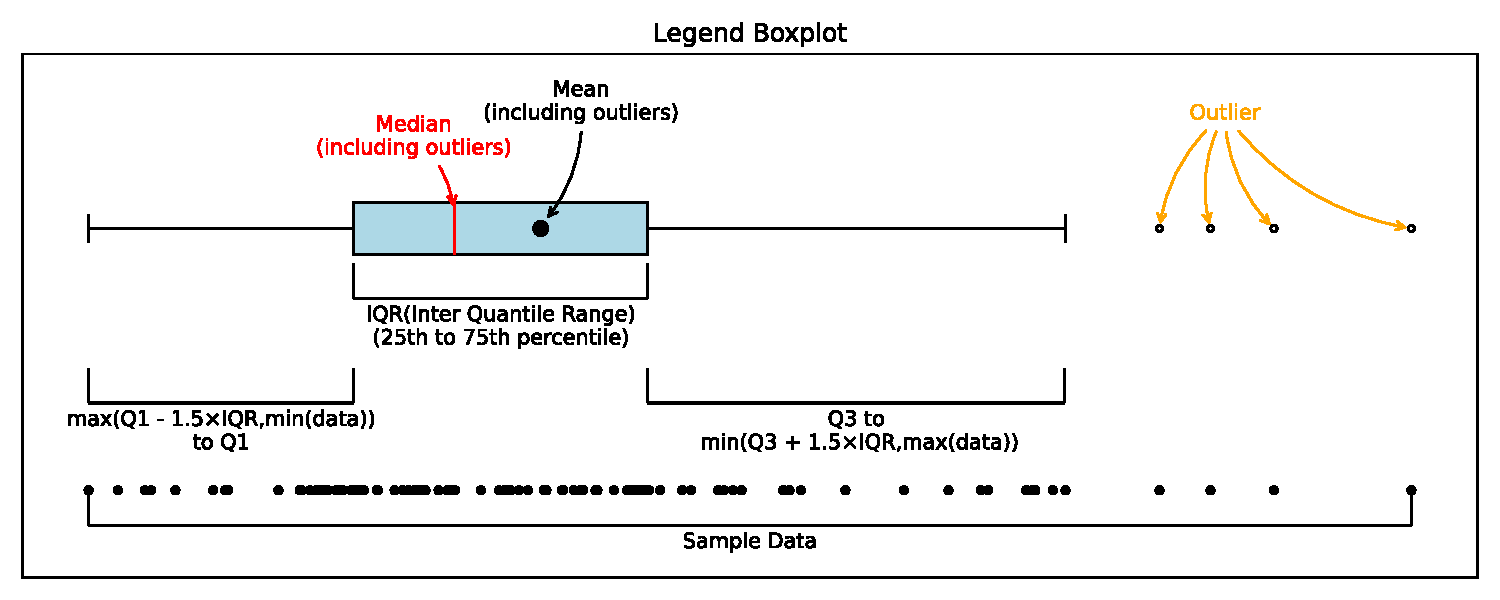
\includegraphics[width=1.\textwidth]{chapters/foundations/images_foundation/legend_boxplot}
    \caption{A boxplot showing the distribution of a toy data set with the important features labeled. Note that the left whiskers is shorted, which indicates that the data is right skewed. Q1 and Q3 denote the 25\% and 75\% quantiles.}\label{fig:boxplots_legends}
\end{figure}